\section{Experiments}

% As with other methods, we observe that introducing a silhouette term into the network loss before the model's pose has been somewhat solved can result in unsatisfactory local minima. We overcome this by using a pre-training stage with the following loss terms:


In this section we compare our method to competitive baselines. We begin by describing our new large-scale dataset of annotated dog images, followed by a quantitative and qualitative evaluation.

\subsection{Evaluation protocol}

Our evaluation is based on our new StanfordExtra dataset. In line with other methods which tackle ``in-the-wild'' 3D reconstruction of articulated subjects~\cite{kolotouros19learning,kolotouros19convolutional}, we filter images from the original dataset of 20,580 for which the majority of dog keypoints are invisible. We consider these images unsuitable for our full-body dog reconstruction task. We also remove images for which the consistency in keypoint/silhouette segmentations between the 3 annotators is below a set threshold. This leaves us with 8,476 images which we divide per-breed into an 80\%/20\% train and test split.

We consider two primary evaluation metrics. IoU is the intersection-over-union of the projected model silhouette compared to the ground truth annotation and indicates the quality of the reconstructed 3D shape. Percentage of Correct Keypoints (PCK) computes the percentage of joints which are within a normalized distance (based on square root of 2D silhouette area) to the ground truth locations, and evaluates the quality of reconstructed 3D pose. We also produce PCK results on various joint groups (legs, tail, ears, face) to compare the reconstruction accuracy for different parts of the dog model.

% TODO: Incoporate this!
% \subsection{Probability of Keypoints Max (PCK-MAX)} \label{sec:pckmax}

% In this section, we compare reprojected 2D joint accuracy using the \emph{PCK-MAX} evaluation metric. This protocol is similar to the Percentage of Correct Keypoints (PCK) metric~\cite{yang2013articulated} used in the main paper by incoporating `invisible' ground-truth points. The standard PCK metric ignores these points, meaning even correct 3D reconstructions will receive no credit. PCK-MAX instead assumes reconstructed 3D points for missing ground-truth data are correct, providing an interesting upper bound. Results are shown in Table~\ref{tab:baselines} and Table~\ref{tab:animalpose}.

\subsection{Training procedure}

We train our model in two stages. The first omits the silhouette loss which we find can lead the network to unsatisfactory local minima if applied too early. With the silhouette loss turned off, we find it satisfactory to use the simple unimodal prior (and without EM) for this preliminary stage since there is no loss to specifically encourage a strong shape alignment. After this, we introduce the silhouette loss, the mixture prior and begin applying the expectation maximization updates over $M=10$ clusters. We train the first stage for 250 epochs, the second stage for 150 and apply the EM step every 50 epochs. The entire training procedure takes 96 hours on a single P100 GPU.

Recall that the training objective for our end-to-end system for predicting SMBLD parameters consistent with a monocular dog input image is given by:

\begin{equation}
    \L{opt}=\L{joints}+\L{sil}+\L{pose}+\L{shape}+\L{mixture}
\end{equation}

Each loss term is weighted with a scalar $\W{}$ and we train our method in two stages:

\ss{Stage 1.} We set $\W{joints}=10.0,\W{pose}=1.0,\W{shape}=1.0,\W{sil}=0.0,\W{mixture}=0.0$. We train this stage for 250 epochs, using the Adam optimizer, with learning rate set to $10^{-4}$. 
\ss{Stage 2.} In this stage, we introduce the silhouette loss to encourage a shape alignment between the projected model silhouette and the ground truth annotation. We set $\W{joints}=10.0,\W{pose}=0.5,\W{shape}=0.0,\W{sil}=100.0,\W{mixture}=0.1$. We train this stage for 150 epochs and run the described EM update step every $K=15$ epochs. We selected to use $M=10$ clusters based on a grid search over $M=1,5,10,25$ and comparing IoU. We again use the Adam optimizer, and set the learning rate to $10^{-5}$.

\subsection{Comparison to baselines}

We first compare our method to various baseline methods. SMAL~\cite{zuffi2017menagerie} is an approach which fits the 3D SMAL model using per-image energy minimization. Creatures Great and SMAL (CGAS)~\cite{biggs2018creatures} is a three-stage method, which employs a joint predictor on silhouette renderings from synthetic 3D dogs, applies a genetic algorithm to clean predictions, and finally applies the SMAL optimizer to produce the 3D mesh.

At test-time both SMAL and CGAS rely on manually-provided segementation masks, and SMAL also relies on hand-clicked keypoints. In order to produce a fair comparison, we produce a set of \emph{predicted} keypoints for StanfordExtra by training the Stacked Hourglass Network~\cite{newell2016stacked} with 8 stacks and 1 block, and \emph{predicted} segmentation masks using DeepLab v3+~\cite{deeplabv3plus}. The Stacked Hourglass Network achieves 71.4\% PCK score, DeepLab v3+ achieves 83.4\% IoU score and the CGAS joint predictor achieves 41.8\% PCK score. 

%All methods are trained from scratch and evaluated on our Stanford Dog validation set.

Table~\ref{tab:baselines} and Figure~\ref{fig:comparison_sup} show the comparison against competitive methods. For full examination, we additionally provide results for SMAL and CGAS in the scenario that ground-truth keypoints and/or segmentations are available at test time. 

The results show our end-to-end method outperforms the competitors when they are provided with predicted keypoints/segmentations (white rows). Our method therefore achieves a new state of the art on this 3D reconstruction task. In addition, we show our method achieves improved average IoU/PCK scores than competitive methods, even when they are provided ground truth annotations at test time (grey rows). We also demonstrate wider applicability of two contributions from our work (scale parameters and improved prior) by showing improved performance of the SMAL method when these are incorporated. Finally, our model's test-time speed is significantly faster than the competitors as it does not require an optimizer.

\begin{table}[]
{
    \small
    \centering
    \begin{tabular}{@{}lcccccccc@{}}
    \toprule
    \multicolumn{1}{l}{Method} & 
    \multicolumn{1}{c}{Kps} & 
    \multicolumn{1}{c}{Seg} & 
    \multicolumn{1}{c}{IoU} & 
    \multicolumn{5}{c}{PCK} \\
    \multicolumn{4}{c}{} &
    \multicolumn{1}{c}{Avg} &
    \multicolumn{1}{c}{Legs} &
    \multicolumn{1}{c}{Tail} &
    \multicolumn{1}{c}{Ears} &
    \multicolumn{1}{c}{Face} \\
    \midrule
    SMAL~\cite{zuffi2017menagerie} & Pred & Pred & 67.9 & 67.1 & 65.7 & 79.5 & 54.9 & 87.4  \\
    SMAL & GT & GT &  69.2 & 72.6 & 69.9 & \textbf{92.0} & 58.6 & \textbf{96.9} \\
    SMAL & GT & Pred & 68.6 & 72.6 & 70.2 & 91.5 & 58.1 & \textbf{96.9} \\ 
    SMAL & Pred & GT & 68.5 & 67.4 & 66.0 & 79.9 & 55.0 & 88.2 \\ 
    % \rowcolor[gray]{.9} SMAL & GT & GT &  69.2 & 72.6 & 69.9 & \textbf{92.0} & 58.6 & \textbf{96.9} \\
    % \rowcolor[gray]{.9} SMAL & GT & Pred & 68.6 & 72.6 & 70.2 & 91.5 & 58.1 & \textbf{96.9} \\ 
    % \rowcolor[gray]{.9} SMAL & Pred & GT & 68.5 & 67.4 & 66.0 & 79.9 & 55.0 & 88.2 \\ 
    \hline
    CGAS~\cite{biggs2018creatures} & CGAS & Pred & 62.4 & 43.7 & 46.5 & 64.1 & 36.5 & 21.4  \\
    % \rowcolor[gray]{.9} CGAS & CGAS & GT & 63.1 & 43.6 & 46.3 & 64.2 & 36.3 & 21.6 \\
    CGAS & CGAS & GT & 63.1 & 43.6 & 46.3 & 64.2 & 36.3 & 21.6 \\
    \hline
    % \rowcolor[gray]{.9} SMAL + scaling & Pred & Pred & 69.3 & 69.6 & 69.4 & 79.3 & 56.5 & 87.6 \\
    % \rowcolor[gray]{.9} SMAL + scaling + new prior & Pred & Pred & 70.7 & 71.6 & 71.5 & 80.7 & 59.3 & 88.0 \\
    SMAL + scaling & Pred & Pred & 69.3 & 69.6 & 69.4 & 79.3 & 56.5 & 87.6 \\
    SMAL + scaling + new prior & Pred & Pred & 70.7 & 71.6 & 71.5 & 80.7 & 59.3 & 88.0 \\
    \hline
    \textbf{Ours} & --- & --- & \textbf{73.6} & \textbf{75.7} & \textbf{75.0} & 77.6 & \textbf{69.9} & 90.0 \\
    \bottomrule 
    \end{tabular}
    \vspace{1em}
    \caption{\label{tab:baselines}\textbf{Baseline comparisons.} Both PCK and silhouette IOU scores are shown for SOTA methods under varying conditions. A combination of both ground truth (GT) and predicted (Pred) keypoints/segmentations using hourglass network and deeplab respectively. For the CGAS method we also test using their keypoint predictor (CGAS). The addition of scaling and new prior are shown to improve the original SMAL method.}
}
\end{table}
\newcolumntype{?}{!{\vrule width 1pt}}

% \newcommand\sfac{0.082}
% \newcommand\spacercomp{4mm}
\begin{figure*}[ht!]
    \centering
    \setkeys{Gin}{width=\linewidth}
    \renewcommand\tabularxcolumn[1]{>{\Centering}m{\sfac\linewidth}} % set all columns to be centered v & hwise, with a fixed length
    % \begin{tabularx}{\textwidth}{c*{5}{X}@{\hspace{\spacercomp}}*{5}{X}c}
    \begin{tabularx}{\textwidth}{c*{5}{X}}
      \textbf{Ours} &
      \includegraphics{ours_sup/n02086646-Blenheim_spaniel/orig/n02086646_1476.jpg} &
      \includegraphics{ours_sup/n02086646-Blenheim_spaniel/fit/n02086646_1476.jpg} &
      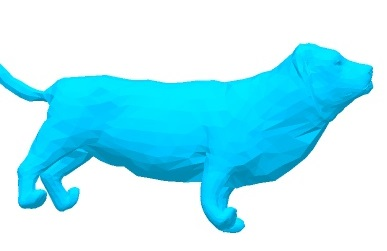
\includegraphics{ours_sup/n02086646-Blenheim_spaniel/model/n02086646_1476_crop.jpg} &
      \includegraphics{ours_sup/n02086646-Blenheim_spaniel/joints/n02086646_1476.jpg} &
      \includegraphics{ours_sup/n02086646-Blenheim_spaniel/segs/n02086646_1476.jpg} \\
      

      3D-M &
      \includegraphics{comp_sup/smal/n02086646-Blenheim_spaniel/orig/n02086646_1476.jpg} &
      \includegraphics{comp_sup/smal/n02086646-Blenheim_spaniel/fit/n02086646_1476.jpg} &
      \includegraphics{comp_sup/smal/n02086646-Blenheim_spaniel/model/n02086646_1476_fixed_crop.jpg} &
      \includegraphics{comp_sup/smal/n02086646-Blenheim_spaniel/joints/n02086646_1476.jpg} &
      \includegraphics{comp_sup/smal/n02086646-Blenheim_spaniel/segs/n02086646_1476.jpg} \\
      


      CGAS &
      \includegraphics{comp_sup/cgas/n02086646-Blenheim_spaniel/orig/n02086646_1476.jpg} &
      \includegraphics{comp_sup/cgas/n02086646-Blenheim_spaniel/fit/n02086646_1476.jpg} &
      \includegraphics{comp_sup/cgas/n02086646-Blenheim_spaniel/model/n02086646_1476_fixed_crop.jpg} &
      \includegraphics{comp_sup/cgas/n02086646-Blenheim_spaniel/joints/n02086646_1476.jpg} &
      \includegraphics{comp_sup/cgas/n02086646-Blenheim_spaniel/segs/n02086646_1476.jpg} \\
      %\hspace{\spacercomp}
     
      \textbf{Ours} &
      \includegraphics{ours_sup/n02087394-Rhodesian_ridgeback/orig/n02087394_831.jpg} &
      \includegraphics{ours_sup/n02087394-Rhodesian_ridgeback/fit/n02087394_831.jpg} &
      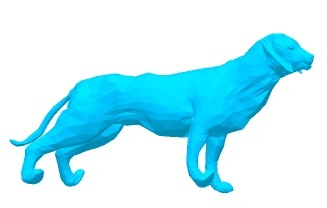
\includegraphics{ours_sup/n02087394-Rhodesian_ridgeback/model/n02087394_831_crop.jpg} &
      \includegraphics{ours_sup/n02087394-Rhodesian_ridgeback/joints/n02087394_831.jpg} &
      \includegraphics{ours_sup/n02087394-Rhodesian_ridgeback/segs/n02087394_831.jpg} \\

      3D-M &
      %\hspace{\spacercomp}
      \includegraphics{comp_sup/smal/n02087394-Rhodesian_ridgeback/orig/n02087394_831.jpg} &
      \includegraphics{comp_sup/smal/n02087394-Rhodesian_ridgeback/fit/n02087394_831.jpg} &
      \includegraphics{comp_sup/smal/n02087394-Rhodesian_ridgeback/model/n02087394_831_fixed_crop.jpg} &
      \includegraphics{comp_sup/smal/n02087394-Rhodesian_ridgeback/joints/n02087394_831.jpg} &
      \includegraphics{comp_sup/smal/n02087394-Rhodesian_ridgeback/segs/n02087394_831.jpg} \\

      CGAS &
      \includegraphics{comp_sup/cgas/n02087394-Rhodesian_ridgeback/orig/n02087394_831.jpg} &
      \includegraphics{comp_sup/cgas/n02087394-Rhodesian_ridgeback/fit/n02087394_831.jpg} &
      \includegraphics{comp_sup/cgas/n02087394-Rhodesian_ridgeback/model/n02087394_831_fixed_crop.jpg} &
      \includegraphics{comp_sup/cgas/n02087394-Rhodesian_ridgeback/joints/n02087394_831.jpg} &
      \includegraphics{comp_sup/cgas/n02087394-Rhodesian_ridgeback/segs/n02087394_831.jpg} \\
      
      \textbf{Ours} &
      \includegraphics{ours_sup/n02091134-whippet/orig/n02091134_16201.jpg} &
      \includegraphics{ours_sup/n02091134-whippet/fit/n02091134_16201.jpg} &
      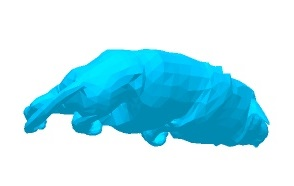
\includegraphics{ours_sup/n02091134-whippet/model/n02091134_16201_crop.jpg} &
      \includegraphics{ours_sup/n02091134-whippet/joints/n02091134_16201.jpg} &
      \includegraphics{ours_sup/n02091134-whippet/segs/n02091134_16201.jpg} \\


      3D-M & 
      \includegraphics{comp_sup/smal/n02091134-whippet/orig/n02091134_16201.jpg} &
      \includegraphics{comp_sup/smal/n02091134-whippet/fit/n02091134_16201.jpg} &
      \includegraphics{comp_sup/smal/n02091134-whippet/model/n02091134_16201_fixed_crop.jpg} &
      \includegraphics{comp_sup/smal/n02091134-whippet/joints/n02091134_16201.jpg} &
      \includegraphics{comp_sup/smal/n02091134-whippet/segs/n02091134_16201.jpg} \\
      
      
      CGAS &
      \includegraphics{comp_sup/cgas/n02091134-whippet/orig/n02091134_16201.jpg} &
      \includegraphics{comp_sup/cgas/n02091134-whippet/fit/n02091134_16201.jpg} &
      \includegraphics{comp_sup/cgas/n02091134-whippet/model/n02091134_16201_fixed_crop.jpg} &
      \includegraphics{comp_sup/cgas/n02091134-whippet/joints/n02091134_16201.jpg} &
      \includegraphics{comp_sup/cgas/n02091134-whippet/segs/n02091134_16201.jpg} \\

      \textbf{Ours} &
      \includegraphics{ours_sup/n02089078-black-and-tan_coonhound/orig/n02089078_877.jpg} &
      \includegraphics{ours_sup/n02089078-black-and-tan_coonhound/fit/n02089078_877.jpg} &
      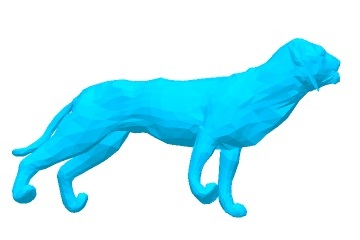
\includegraphics{ours_sup/n02089078-black-and-tan_coonhound/model/n02089078_877_crop.jpg} &
      \includegraphics{ours_sup/n02089078-black-and-tan_coonhound/joints/n02089078_877.jpg} &
      \includegraphics{ours_sup/n02089078-black-and-tan_coonhound/segs/n02089078_877.jpg} \\

      3D-M & 
      \includegraphics{comp_sup/smal/n02089078-black-and-tan_coonhound/orig/n02089078_877.jpg}&
      \includegraphics{comp_sup/smal/n02089078-black-and-tan_coonhound/fit/n02089078_877.jpg}&
      \includegraphics{comp_sup/smal/n02089078-black-and-tan_coonhound/model/n02089078_877_fixed_crop.jpg}&
      \includegraphics{comp_sup/smal/n02089078-black-and-tan_coonhound/joints/n02089078_877.jpg}&
      \includegraphics{comp_sup/smal/n02089078-black-and-tan_coonhound/segs/n02089078_877.jpg} \\
      
      CGAS &
      \includegraphics{comp_sup/cgas/n02089078-black-and-tan_coonhound/orig/n02089078_877.jpg}&
      \includegraphics{comp_sup/cgas/n02089078-black-and-tan_coonhound/fit/n02089078_877.jpg}&
      \includegraphics{comp_sup/cgas/n02089078-black-and-tan_coonhound/model/n02089078_877_fixed_crop.jpg}&
      \includegraphics{comp_sup/cgas/n02089078-black-and-tan_coonhound/joints/n02089078_877.jpg}&
      \includegraphics{comp_sup/cgas/n02089078-black-and-tan_coonhound/segs/n02089078_877.jpg} \\

      % \textbf{Ours} &
      % \includegraphics{ours_sup/n02087394-Rhodesian_ridgeback/orig/n02087394_831.jpg} &
      % \includegraphics{ours_sup/n02087394-Rhodesian_ridgeback/fit/n02087394_831.jpg} &
      % \includegraphics{ours_sup/n02087394-Rhodesian_ridgeback/model/n02087394_831.jpg} &
      % \includegraphics{ours_sup/n02087394-Rhodesian_ridgeback/joints/n02087394_831.jpg} &
      % \includegraphics{ours_sup/n02087394-Rhodesian_ridgeback/segs/n02087394_831.jpg} &
      % %\hspace{\spacercomp}


      % SMAL &
      % \includegraphics{comp_sup/smal/n02087394-Rhodesian_ridgeback/orig/n02087394_831.jpg} &
      % \includegraphics{comp_sup/smal/n02087394-Rhodesian_ridgeback/fit/n02087394_831.jpg} &
      % \includegraphics{comp_sup/smal/n02087394-Rhodesian_ridgeback/model/n02087394_831.jpg} &
      % \includegraphics{comp_sup/smal/n02087394-Rhodesian_ridgeback/joints/n02087394_831.jpg} &
      % \includegraphics{comp_sup/smal/n02087394-Rhodesian_ridgeback/segs/n02087394_831.jpg} &
      % %\hspace{\spacercomp}
      % \includegraphics{comp_sup/smal/n02089078-black-and-tan_coonhound/orig/n02089078_877.jpg} &
      % \includegraphics{comp_sup/smal/n02089078-black-and-tan_coonhound/fit/n02089078_877.jpg} &
      % \includegraphics{comp_sup/smal/n02089078-black-and-tan_coonhound/model/n02089078_877.jpg} &
      % \includegraphics{comp_sup/smal/n02089078-black-and-tan_coonhound/joints/n02089078_877.jpg} &
      % \includegraphics{comp_sup/smal/n02089078-black-and-tan_coonhound/segs/n02089078_877.jpg} \\

      % CGAS &
      % \includegraphics{comp_sup/cgas/n02087394-Rhodesian_ridgeback/orig/n02087394_831.jpg} &
      % \includegraphics{comp_sup/cgas/n02087394-Rhodesian_ridgeback/fit/n02087394_831.jpg} &
      % \includegraphics{comp_sup/cgas/n02087394-Rhodesian_ridgeback/model/n02087394_831.jpg} &
      % \includegraphics{comp_sup/cgas/n02087394-Rhodesian_ridgeback/joints/n02087394_831.jpg} &
      % \includegraphics{comp_sup/cgas/n02087394-Rhodesian_ridgeback/segs/n02087394_831.jpg} &
      % %\hspace{\spacercomp}
      % \includegraphics{comp_sup/cgas/n02089078-black-and-tan_coonhound/orig/n02089078_877.jpg} &
      % \includegraphics{comp_sup/cgas/n02089078-black-and-tan_coonhound/fit/n02089078_877.jpg} &
      % \includegraphics{comp_sup/cgas/n02089078-black-and-tan_coonhound/model/n02089078_877.jpg} &
      % \includegraphics{comp_sup/cgas/n02089078-black-and-tan_coonhound/joints/n02089078_877.jpg} &
      % \includegraphics{comp_sup/cgas/n02089078-black-and-tan_coonhound/segs/n02089078_877.jpg} \\

      % \textbf{Ours} &
      % \includegraphics{ours_sup/n02085936-Maltese_dog/orig/n02085936_3313.jpg} &
      % \includegraphics{ours_sup/n02085936-Maltese_dog/fit/n02085936_3313.jpg} &
      % \includegraphics{ours_sup/n02085936-Maltese_dog/model/n02085936_3313.jpg} &
      % \includegraphics{ours_sup/n02085936-Maltese_dog/joints/n02085936_3313.jpg} &
      % \includegraphics{ours_sup/n02085936-Maltese_dog/segs/n02085936_3313.jpg} &
      % %\hspace{\spacercomp}
      % \includegraphics{ours_sup/n02088238-basset/orig/n02088238_10054.jpg} &
      % \includegraphics{ours_sup/n02088238-basset/fit/n02088238_10054.jpg} &
      % \includegraphics{ours_sup/n02088238-basset/model/n02088238_10054.jpg} &
      % \includegraphics{ours_sup/n02088238-basset/joints/n02088238_10054.jpg} &
      % \includegraphics{ours_sup/n02088238-basset/segs/n02088238_10054.jpg} \\

      % SMAL &
      % \includegraphics{comp_sup/smal/n02085936-Maltese_dog/orig/n02085936_3313.jpg} &
      % \includegraphics{comp_sup/smal/n02085936-Maltese_dog/fit/n02085936_3313.jpg} &
      % \includegraphics{comp_sup/smal/n02085936-Maltese_dog/model/n02085936_3313.jpg} &
      % \includegraphics{comp_sup/smal/n02085936-Maltese_dog/joints/n02085936_3313.jpg} &
      % \includegraphics{comp_sup/smal/n02085936-Maltese_dog/segs/n02085936_3313.jpg} &
      % %\hspace{\spacercomp}
      % \includegraphics{comp_sup/smal/n02088238-basset/orig/n02088238_10054.jpg} &
      % \includegraphics{comp_sup/smal/n02088238-basset/fit/n02088238_10054.jpg} &
      % \includegraphics{comp_sup/smal/n02088238-basset/model/n02088238_10054.jpg} &
      % \includegraphics{comp_sup/smal/n02088238-basset/joints/n02088238_10054.jpg} &
      % \includegraphics{comp_sup/smal/n02088238-basset/segs/n02088238_10054.jpg} \\

      % CGAS &
      % \includegraphics{comp_sup/cgas/n02085936-Maltese_dog/orig/n02085936_3313.jpg} &
      % \includegraphics{comp_sup/cgas/n02085936-Maltese_dog/fit/n02085936_3313.jpg} &
      % \includegraphics{comp_sup/cgas/n02085936-Maltese_dog/model/n02085936_3313.jpg} &
      % \includegraphics{comp_sup/cgas/n02085936-Maltese_dog/joints/n02085936_3313.jpg} &
      % \includegraphics{comp_sup/cgas/n02085936-Maltese_dog/segs/n02085936_3313.jpg} &
      % %\hspace{\spacercomp}
      % \includegraphics{comp_sup/cgas/n02088238-basset/orig/n02088238_10054.jpg} &
      % \includegraphics{comp_sup/cgas/n02088238-basset/fit/n02088238_10054.jpg} &
      % \includegraphics{comp_sup/cgas/n02088238-basset/model/n02088238_10054.jpg} &
      % \includegraphics{comp_sup/cgas/n02088238-basset/joints/n02088238_10054.jpg} &
      % \includegraphics{comp_sup/cgas/n02088238-basset/segs/n02088238_10054.jpg} \\

      % & 
      & (a) & (b) & (c) & (d) & (e) \\
      %\hspace{\spacercomp} 
      % (a) & (b) & (c) & (d) & (e) \\
    \end{tabularx}
    %
    \caption{%
    \textbf{Qualitiative comparison to SOTA.} 
    Row 1: \textbf{Ours}, 
    Row 2: 3D-M~\cite{zuffi2017menagerie}, 
    Row 3: CGAS~\cite{biggs2018creatures}. 
    (a) input image, (b) predicted 3D mesh, (c) canonical view 3D mesh, 
    (d) reprojected model joints and (e) silhouette reprojection error. 
    }
    \label{fig:comparison_sup}
\end{figure*}


%xxx: Note that CGAS does badly as it can't clean up using video
\subsection{Generalization to unseen dataset}

Table~\ref{tab:animalpose} shows an experiment to compare how well our model generalizes to a new data domain. We test our model against the SMAL~\cite{zuffi2017menagerie} method (using predicted keypoints and segmentations as above for fairness) on the recent Animal Pose dataset~\cite{animalpose}. The data preparation process is the same as for StanfordExtra and no fine-tuning was used for either method. We achieve good results in this unseen domain and still improve over the SMAL optimizer.

\begin{table}
\begin{tabular}{@{}lcccccc@{}}
\toprule
\multicolumn{1}{l}{Method} & 
\multicolumn{1}{c}{IoU} & 
\multicolumn{5}{c}{PCK} \\
\multicolumn{2}{c}{} &
\multicolumn{1}{c}{Avg} &
\multicolumn{1}{c}{Legs} &
\multicolumn{1}{c}{Tail} &
\multicolumn{1}{c}{Ears} &
\multicolumn{1}{c}{Face} \\
\midrule
SMAL~\cite{zuffi2017menagerie} & 63.6 & 69.1 & 60.9 & 83.5 & 75.0 & 93.0 \\
% \hline
\textbf{Ours} & \textbf{66.9} & \textbf{73.8} & \textbf{65.1} & \textbf{85.6} & \textbf{84.0} & \textbf{93.6} \\
\bottomrule
\multicolumn{7}{c}{} \\
\multicolumn{7}{c}{}
% \textbf{Ours} & \textbf{66.9} & \textbf{73.8} & \textbf{65.1} & \textbf{85.6} & \textbf{84.0} & \textbf{93.6} \\
% \textbf{Ours} & \textbf{66.9} & \textbf{73.8} & \textbf{65.1} & \textbf{85.6} & \textbf{84.0} & \textbf{93.6}

\end{tabular}
\caption{
    \label{tab:animalpose}
    \textbf{Animal Pose dataset~\cite{animalpose}}. Evaluation on recent Animal Pose dataset with no fine-tuning to our method nor joint/silhouette predictors used for SMAL.}
\end{table}

\begin{table}
\begin{tabular}{@{}lcccccc@{}}
\toprule
\multicolumn{1}{l}{Method} & 
\multicolumn{1}{c}{IoU} & 
\multicolumn{5}{c}{PCK} \\
\multicolumn{2}{c}{} &
\multicolumn{1}{c}{Avg} &
\multicolumn{1}{c}{Legs} &
\multicolumn{1}{c}{Tail} &
\multicolumn{1}{c}{Ears} &
\multicolumn{1}{c}{Face} \\
\midrule
\textbf{Ours} & \textbf{73.6} & \textbf{75.7} & \textbf{75.0} & \textbf{77.6} & 69.9 & 90.0 \\
$-$EM & 67.7 & 74.6 & 72.9 & 75.2 & \textbf{72.5} & 88.3 \\
$-$MoG & 68.0 & 74.9 & 74.3 & 73.3 & 70.0 & \textbf{90.2} \\ 
$-$Scale & 67.3 & 72.6 & 72.9 & 75.3 & 62.3 & 89.1 \\
\bottomrule 
\end{tabular}
\caption{\label{tab:ablation}\textbf{Ablation study.} Evaluation with the following contributions removed: (a) EM updates, (b) Mixture Shape Prior, (c) SMBLD scale parameters.}
\end{table}


\subsection{Ablation study}

We also produce a study in which we ablate individual components of our method and examine the effect on the PCK/IoU performance. We evaluate three variants: (1) \textbf{Ours w/o EM} that omits EM updates, (2) \textbf{Ours w/o MoG} which replaces our mixture shape prior with a unimodal prior, (3)~\textbf{Ours w/o Scale} which removes the scale parameters. 

The results in Table~\ref{tab:ablation} indicate that each individual component has a positive impact on the overall method performance. In particular, it can be seen that the inclusion of the EM and Mixture of Gaussians prior leads to an improvement in IoU, suggesting that the shape prior refinements steps help the model accurately fit the exact dog shape. Interestingly, we notice that adding the Mixture of Gaussians prior but omitting EM steps slightly hinders performance, perhaps due to an sub-optimal initialization for the $M$ clusters. However, we find adding EM updates to the Mixture of Gaussian model improves all metrics except the ear keypoint accuracy. We observe the error here is caused by the our shape prior learning slightly imprecise shapes for dogs with extremely ``floppy'' ears. Although there is good silhouette coverage for these regions, the fact our model has only a single articulation point per ear causes a lack of flexibility that results in occasionally misplaced ear tips for these instances. This could be improved in future work by adding additional model joints to the ear. Finally, we find the increased model flexibility afforded by the SMBLD scale parameters have a positive effect on IoU/PCK scores. 


% We are able to use the dataset to examine which dog parts are the most challenging to position. 
% \input{eccv2020kit/fig_jointspreads}
% \anote{TODO: PCK tables and errors visualized on 3D dog.}
% \paragraph{Analysis over breeds}
% A significant benefit of our dog dataset is that the supplied breed labels allows for reconstruction performance to be evaluated over particular breeds. \anote{Figure} ranks the breeds by error.
% \begin{table}[]
\small
\centering
\begin{tabular}{@{}lrrrr@{}}
\toprule
\multicolumn{1}{l}{} & 
\multicolumn{1}{c}{PCK}         & 
\multicolumn{1}{c}{IoU}         & 
\multicolumn{1}{c}{Metric 3}         & 
\multicolumn{1}{c}{Metric 4}          
\\ \midrule
\multicolumn{1}{r}{Daschund}             & 109.1                    & 99.6                     & 96.5                     & 95.5                     \\

\end{tabular}
\vspace{1em}
\caption{\label{tab:breed}\textbf{Evaluation of breeds} showing that there is a difference}
\end{table}

\subsection{Qualitative evaluation}

Figure~\ref{fig:comparison_sup} shows a range of example system outputs when tested on range of StanfordExtra and Animal Pose~\cite{animalpose} dogs with varying pose and shape and in challenging conditions. Note that only StanfordExtra is used for training.


% \input{fig_comparison}

% \input{fig_qualresults}

% \input{fig_qual_results_animal_pose}
% \section{Failure Cases}